\hypersetup{linkcolor=blue, citecolor=red}

\chapter{Architettura e Progettazione delle Reti Aziendali} \label{chap:2}

\section{Problemi Comuni nelle Reti}
        Alcune reti aziendali, similmente a quelle di pubblico utilizzo come quelle delle università o degli enti pubblici, mettono a disposizione dati o servizi accessibili da chiunque. Questo tipo di infrastrutture sono da sempre le vittime perfette per attacchi distribuiti nella rete, i quali puntano a paralizzare i sistemi informatici. 
        Per mitigare questi attacchi, gli amministratori della rete possono prendere dei provvedimenti utilizzando dei dispositivi come firewall e sistemi di intrusion detection e prevention.
        
        \vspace{2mm}
        
            Ovviamente non sono solo le reti che offrono un servizio di hosting ad 
            avere problemi di sicurezza. Notiamo infatti da questo paper \cite{smb_security_mesures} come la maggior parte delle piccole-medie imprese non implementino in maniera adeguata la sicurezza informatica, diventando semplici vittime di potenziali attaccanti. Secondo questo articolo \cite{sole_24} del Sole 24 Ore, in Italia “le piccole e medie imprese contribuiscono per il 63\% al valore aggiunto e per il 76\% all'occupazione”, mentre in Europa \cite{eu_site_PMI} “si contano oltre 23 milioni di PMI, pari al 99\% delle imprese e due posti di lavoro su tre nel settore privato”. Queste sono dunque un motore chiave 
            dell'economia nella maggior parte dei paesi e dati rubati, esposti o servizi manomessi, risultano in un danno economico per le PMI.

        
        
        \subsection{Tipi di Rete Aziendale e Implicazioni per la sicurezza}

            Ogni tipologia di rete aziendale presenta specifiche vulnerabilità che 
            derivano dalla sua architettura, dalla posizione geografica e dal 
            contesto operativo. Questi fattori influenzano direttamente le 
            strategie di sicurezza adottabili, rendendo fondamentale un approccio 
            mirato alla protezione di ogni tipo di infrastruttura.
            Di seguito i tre tipi principali di reti, con focus sulle vulnerabilità 
            e contromisure specifiche:

            \newpage
            \begin{itemize}
            \item \textbf{LAN}(Local Area Network): copre un'area contenuta come 
            case o uffici. È usata in genere per collegare computer e altri 
            dispositivi all'interno di un'area limitata.

            \subitem \textbf{Rischi}: Le LAN sono particolarmente vulnerabili ad 
            accessi fisici non autorizzati, al broadcast di traffico sensibile e 
            all'utilizzo di dispositivi personali (BYOD) non controllati, che 
            possono introdurre potenziali punti di ingresso per gli attaccanti.

            \subitem \textbf{Contromisure}: Per mitigare questi rischi, è 
            fondamentale implementare misure di segmentazione come le VLAN per 
            isolare i reparti, adottare protocolli di autenticazione come l’802.1X 
            e monitorare continuamente il traffico per rilevare anomalie o 
            comportamenti sospetti, come analizzato in questo articolo~\cite{how_to_print_sec}.

            \subitem \textbf{Esempio Reale}: Stampanti non protette, ad esempio, rappresentano un rischio significativo, in quanto spesso non vengono configurate correttamente, permettendo a eventuali malintenzionati di accedere alla rete aziendale. Come evidenziato da questo articolo \cite{vul_in_printers}, dimostrando quanto sia importante implementare misure di protezione adeguate per dispositivi di questo tipo.\\
            
            Analizzando questo articolo~\cite{printers_hijack} vediamo come 28\,000 stampanti sono state compromesse nel mondo per dimostrare l'importanza della messa in sicurezza di questi dispositivi. Per dimostrare la riuscita dell'esperimento sono stati stampati dei fogli con delle linee guida su come mettere in sicurezza queste stampanti. L'articolo evidenzia come sono riusciti a penetrare in 27,944 stampanti delle 50\,000 previste, ottenendo un successo del 56\% e stimando che su 800\,000 stampanti connesse a internet circa 447\,000 sono insicure.
            
            \item \textbf{WAN}(Wide Area Network): a differenza della LAN è pensata per coprire una vasta area. 
            È utilizzata per collegare le reti locali tra di loro, è quindi in grado di collegare sedi remote.

            \subitem \textbf{Rischi}: I rischi principali per questo tipo di rete sono: l'intercettazione del traffico su collegamenti pubblici, gli attacchi DDoS verso i router perimetrali o le configurazioni errate dei BGP.

            \subitem \textbf{Contromisure}: Le contromisure adottabili sono: la crittografia del traffico tra le reti, usando VPN IPsec o TLS, 
            implementazioni di protocolli sicuri come BGPSec o l'utilizzo di 
            firewall NGFW (Next-Generation Firewall) con filtraggio deep packet inspection \cite{NGFW_IPSec_VPN_WAN}.

             \subitem \textbf{Esempio Reale}: In questo articolo \cite{pwn2own} viene descritto come nella competizione Pwn2Own\footnote{Fonte: Wikipedia (\url{https://it.wikipedia.org/wiki/Pwn2Own})\\Competizione tra hacker con l'obiettivo di trovare delle falle in software e hardware di ultima generazione ritenuti o che erano stati dichiarati privi di vulnerabilità} una squadra ha trovato una vulnerabilità in un router TP-Link, connesso alla WAN che gli ha permesso di inserirsi nella LAN, attaccando successivamente una telecamera Synology.

            \newpage
            
            \item \textbf{Cloud Networks}: può essere visualizzato come una rete virtualizzata ospitata su un servizio cloud, togliendo il peso della gestione e della configurazione all'utilizzatore. Questo tipo di reti sono composte anche da router virtuali, firewall e altri componenti.

            \subitem \textbf{Rischi}: Le problematiche principali sono quella della mal configurazione di gruppi di sicurezza, accessi non autorizzati tramite API key compromesse e attacchi cross-tenant in ambienti multi-tenant \cite{multi_tenant_risks}.

            \subitem \textbf{Contromisure}: Per aggirare i problemi di questo tipo di rete spesso è buona norma usare un approccio “Zero Trust”, con autenticazione multi-fattoriale. L'adozione di un'automazione della sicurezza tramite vari strumenti, come AWS Config per rilevare configurazioni rischiose \cite{aws_config}, e l'utilizzo di una crittografia end-to-end  per dati in transito e a riposo.

            \subitem\textbf{Esempio reale}: Nel 2024, un’azienda ha subito una violazione dati su AWS a causa di un bucket S3 configurato come pubblico \cite{s3_bucket_attack}. L’implementazione di policy IAM granulari ha risolto il problema.
            
            \end{itemize}
            
            \begin{table}[H]
                \begin{center}
                        \begin{tabular}{ |P{22mm}|P{50mm}|P{52mm}|  }
                            \hline
                            \multicolumn{3}{|c|}{Confronto tra le Vulnerabilità} \\
                            \hline
                            Tipo di Rete & Vulnerabilità Critiche & Best Practice di Sicurezza\\
                            \hline
                            LAN & Accesso fisico, ARP Spoofing & VLAN, 802.1X, NAC(Network Access Control)\vspace{2mm}\\
                            \hline
                            WAN & DDoS, BGP hijacking & VPN, BGPsec, NGFW con mitigazione DDoS\\
                            \hline
                            Cloud & Misconfigurazioni IAM/S3 & Zero Trust, automazione strumenti CSPM\\
                             \hline
                        \end{tabular}
                        \caption{Analisi delle vulnerabilità sui vari tipi di rete.}
                        \label{tab_vulnerabilità}
                \end{center}
            \end{table}            

\newpage

            La costruzione di queste reti richiede l'utilizzo di vari componenti hardware, tra cui modem, switch, router, access point, client, server, load balancer, proxy e altri. A questi si affiancano diversi componenti software, principalmente i protocolli di rete, che implementano i livelli astratti dei modelli concettuali per l'architettura delle reti, 
            come il livello fisico, di collegamento (datalink) e di trasporto, che verranno approfonditi successivamente. La scelta di ognuna di queste cose è dettata dal tipo di esigenze che servono e da priorità di sicurezza diverse. Standardizzare le configurazioni e allinearsi a framework come ISO 27001 permette di creare reti sicure by design.

             \begin{figure}[H]
                \centering
                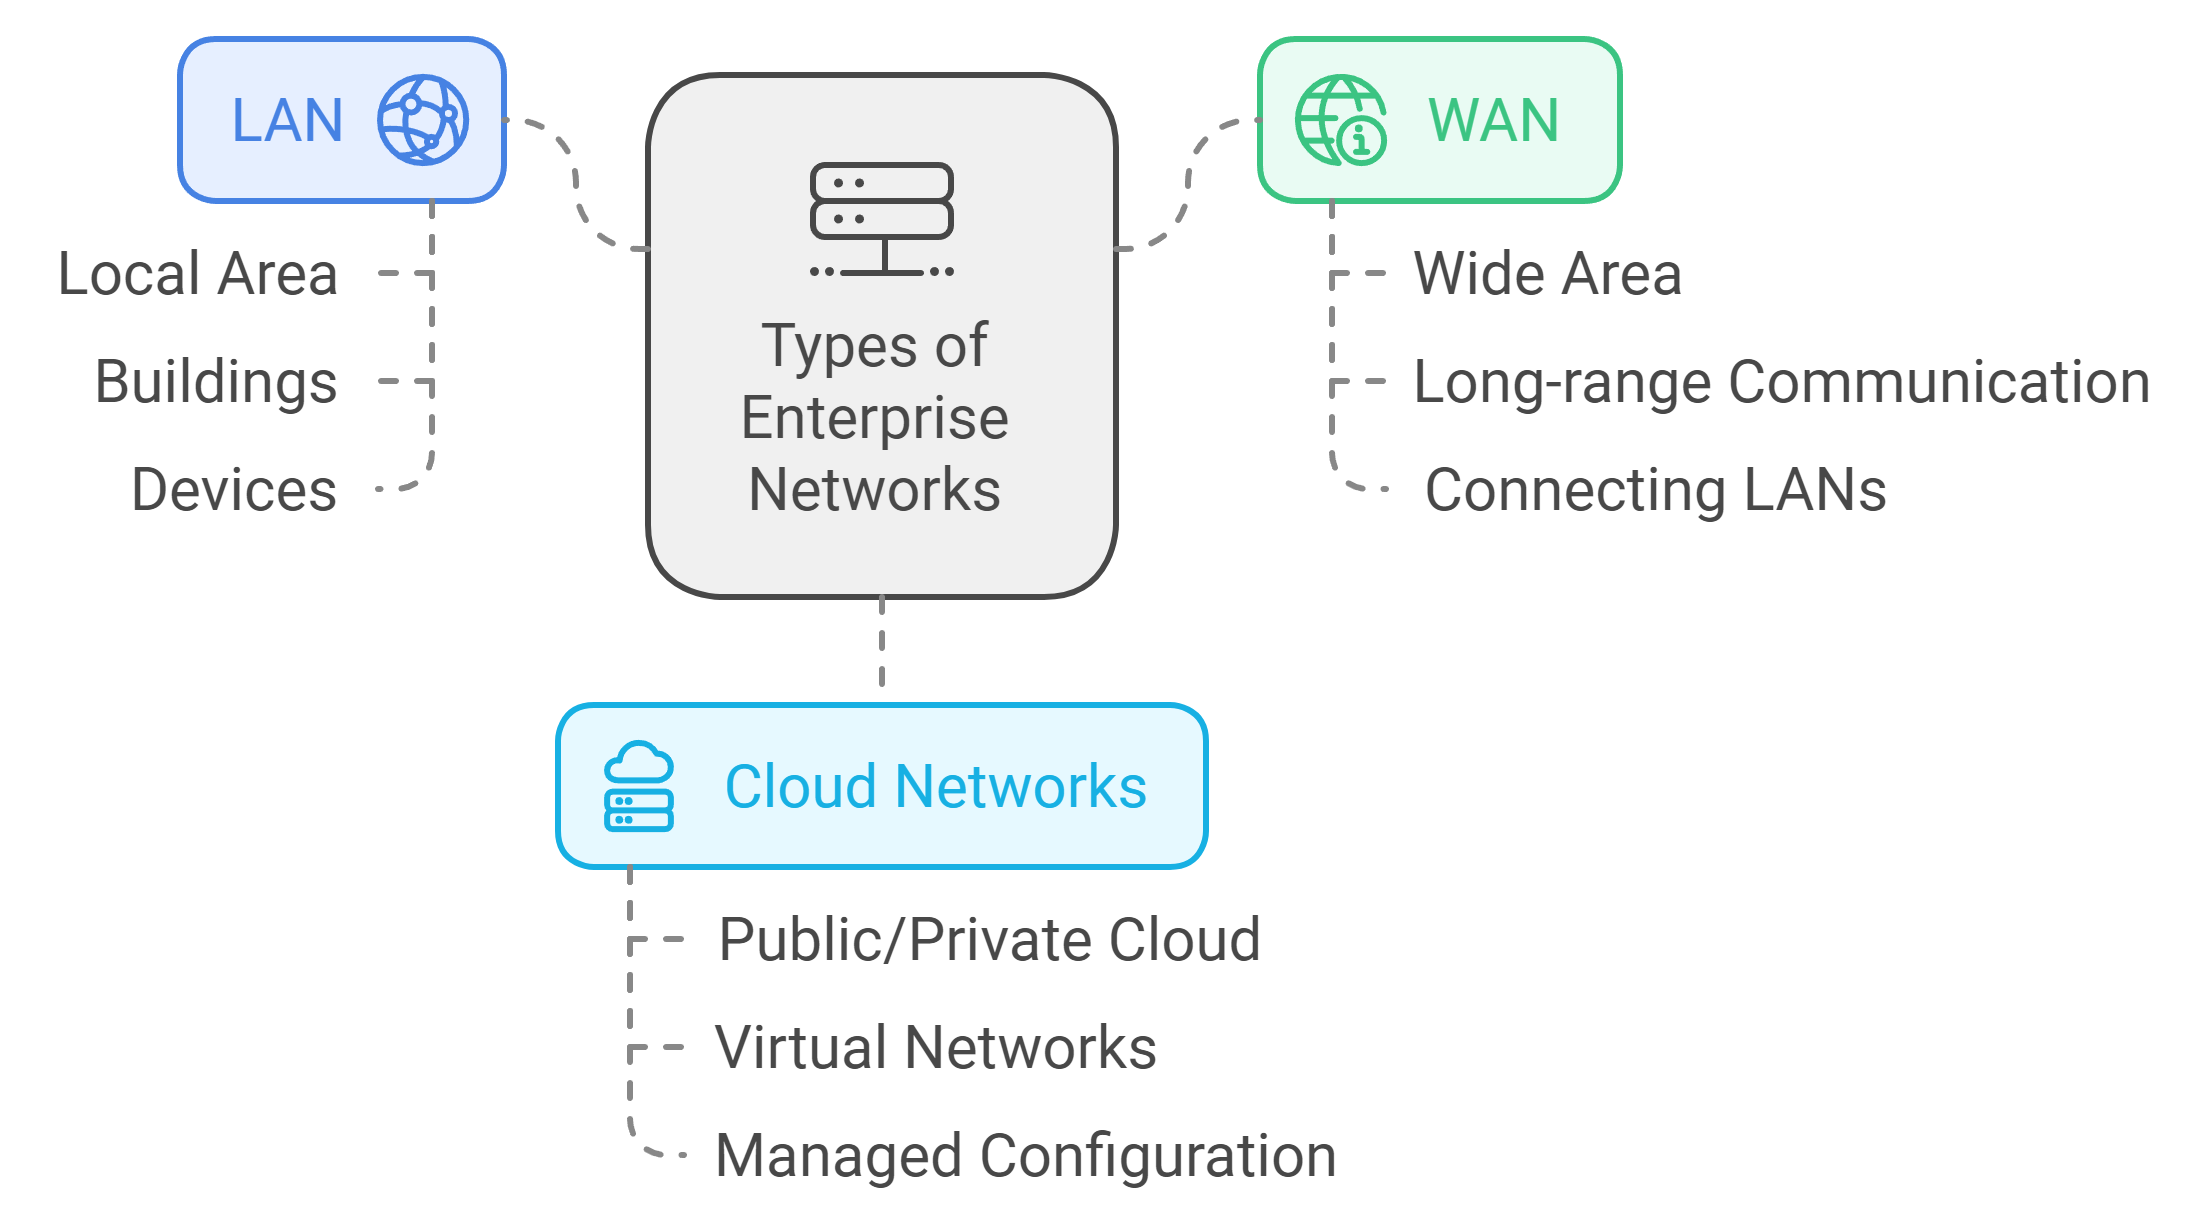
\includegraphics[width=0.6\textwidth]{Immagini/Types_of_net_reppre.png}
                \caption{Rappresentazione dei tipi di Rete.}
                \label{fig:types_of_networks}
            \end{figure}

    \section{Principi e Strumenti per una Progettazione Sicura delle Reti}
            Analizzando il paper \cite{Design_Principles_Secure_Systems} e \cite{Advanced_Networking_Cybersecurity_Approaches}, diamo delle linee guida su qual è lo stato dell'arte da seguire per la progettazione di una rete aziendale sicura, la quale richiede l'integrazione di principi fondamentali come la modularità, l'isolation e il secure-by-default, fondamentali per assicurare un sistema in grado di anticipare le minacce, ridurre la superficie di attacco, garantire resilienza e che si possa recuperare in maniera sicura da fallimenti.

            A partire dal modello “CIA triad”, troviamo tre concetti fondamentali per costruire una rete, e sono: 
            \begin{itemize}
                \item Confidentiality: Protezione di dati sensibili da accessi non autorizzati. Per farlo si usa la crittografia, controllo degli accessi e altre misure.
                \item Integrity: Garanzia che i dati non siano alterati in alcun modo grazie a certificati digitali o a tecniche di hashing
                \item Availability: Possibilità di accedere ai dati e alle risorse quando serve. Per farlo vengono utilizzati sistemi ridondanti o di backup.
            \end{itemize}

            Un sistema sicuro si costruisce a partire da questi tre principi. In base al tipo di attività che si andranno a svolgere con la rete si possono bilanciare alcuni concetti.

            Ci sono poi alcuni principi come l'utilizzo del machine learning, ML, e dell'intelligenza artificiale, di cui parleremo più avanti, che possono aumentare la sicurezza di alcuni sistemi.

            Per difendersi quindi vengono sviluppati algoritmi in grado di rilevare e mitigare problemi di sicurezza in tempo reale, oppure grazie al ML si possono identificare pattern e anomalie.
            È fondamentale scrivere codice in maniera sicura e usare quindi programmi pensati per prevenire attacchi noti come quelli di Buffer overflow, SQL injection, e cross-site scripting.

            Andiamo ora ad approfondire dei punti cardine necessari per costruire un sistema sicuro. È importante ricordare che l'applicazione di queste linee guida si deve adattare alla situazione per cui il sistema verrà usato. 
            Infatti dobbiamo prima stabilire il contesto, gli obiettivi e le potenziali minacce, capire il rischio accettabile e cosa è necessario per eseguire il sistema. Sappiamo che attaccanti poco abili abbandonano l'attacco facilmente dopo qualche tentativo fallito, dobbiamo quindi fare in modo che il sistema 
            sia difficile da attaccare. Bisogna anche prevedere diversi sistemi o livelli di autenticazione in quanto i malintenzionati preferiscono portare a termine i propri attacchi con tecniche di social engineering, email phishing e replay.
            
        
        \subsection{Principio della Difesa in Profondità}
            Per proteggere completamente un sistema non basta un singolo apparato di sicurezza, ma bisogna utilizzare una serie di strumenti e procedure che possono aiutare a fermare gli attacchi in corso e consente all'organizzazione di mitigare una 
            serie di pericoli. 
            Con il principio della difesa in profondità (defense-in-depth) mettiamo le basi per una sicurezza stratificata e ridondante. Se una linea di difesa viene compromessa infatti questo metodo ci permette di limitare i danni nel network; per di più, utilizzare un solo metodo di sicurezza introduce la problematica del “single point of failure” che, se viene compromesso, mette in
            pericolo l'intero sistema. Per implementare questo principio possiamo utilizzare, ad esempio, dei rilevatori. Se un sistema ha due rilevatori, essi possono essere usati in serie o in parallelo in base alla quantità di falsi positivi o negativi ottenuti e in base al sistema richiesto.
        
    
        \vspace{5mm}
            
        \subsection{Principio del Minimo Privilegio}
            Questo principio ci suggerisce di fornire a ogni utente il minimo numero di permessi possibile richiesti per completare il proprio lavoro. Questo principio si applica anche ai programmi usati all'interno di un network, lasciando il numero minimo di permessi necessari per essere eseguito in maniera corretta,
            cercando di minimizzare il livello di privilegi dato a ogni programma.
            

        \subsection{Principio della Separazione dei Poteri}
            L'idea alla base di questo principio è quella di non dare a nessun utente troppo potere su un sistema, anzi il suggerimento è quello di dividere le responsabilità su più utenti, cercando di ridurre così la possibilità di rischi di sicurezza.

        \subsection{Principio della Sicurezza by Default}
            In questo fondamento ci assicuriamo che ogni impostazione di sicurezza sui vari programmi usati sia attiva di default, come:
            \begin{samepage}
                \begin{itemize}
                    \item L'autenticazione a 2 fattori (2FA): meccanismo che richiede due metodi di identificazione all'utente che vuole accedere, e quindi la sola password non sarà sufficiente.
                    \item Crittografia: la crittografia delle informazione permette la lettura dei dati solo da parte di utenti autorizzati.
                    \item Firewall: un dispositivo che permette di controllare il network e restringere il suo traffico basandosi su regole di sicurezza predefinite.
                    \item Secure Boot: una caratteristica dove solo software autorizzato viene caricato all'accensione del sistema.
                \end{itemize}
            \end{samepage}

        \subsection{Principio della Modularità}
            Questo fondamento consiste nello smontare un sistema in piccoli componenti indipendenti o modulabili per aumentare la sicurezza.
            Un esempio di questo principio sono i microservizi, un metodo per sviluppare software modulare dove le grandi applicazioni sono divise in piccoli pezzi e usati indipendentemente. Questa tecnica punta a diminuire la superficie su cui si propaga l'attacco e limita gli effetti di questi. Un altro esempio è quello dell'hardware modulare, dove il sistema è smontato in componenti più piccoli che possono essere facilmente cambiati. Questo incrementa la sicurezza poiché rende più facile identificare problemi nelle patch dei singoli componenti. Un esempio di hardware modulare sono il processore, la RAM e i dispositivi di I/O. Un'altra pratica utilizzata è quella della virtualizzazione, ossia quella tecnologia che permette a più sistemi operativi o applicazioni di essere eseguiti su una singola macchina fisica. Questo aumenta la sicurezza in quanto isola ogni applicazione l'una dall'altra rendendo più difficile per un attaccante spostarsi all'interno del sistema.
            Questa tecnica fornisce un livello di isolamento che permette di limitare l'impatto di un sistema compromesso o può impedire che un
            attacco venga portato a termine.

\newpage
        \subsection{Principio del Fallire in Maniera Sicura}
            Tutti i tipi di sistemi possono fallire, anche i più sicuri. È importante essere preparati a questo tipo di eventi per minimizzare l'impatto e questa strategia è alla base di ogni sistema sicuro di successo. Ci sono alcuni punti da seguire per ottenere ciò:

        \begin{samepage}
            \begin{itemize}
                \item Fallire con grazia (Fail Gracefully): ossia i sistemi e le applicazioni devono essere costruite per questa eventualità così da fare in modo che funzionino il più possibile anche sotto attacco. Per esempio se un sito di un ristorante d'asporto viene compromesso gli utenti devono avere la possibilità di vedere il menù ma no di piazzare ordini.
                \item Accesso Limitato: l'accesso a dati sensibili deve essere limitato solo agli utenti che
                lo necessitano veramente, per minimizzare l'impatto di un possibile attacco.
                \item Test e Aggiornamenti Frequenti: per prevenire le vulnerabilità è importante aggiornare con frequenza un sistema e testarlo con dei metodi di pentesting per assicurarsi della sua sicurezza.
                \item Crittografia: I dati sensibili devono essere crittografati, sia quando vengono mossi (inviati) sia quando vengono solo tenuti in memoria, da accessi non autorizzati.
            \end{itemize}
        \end{samepage}

        \subsection{Principio di Isolamento}
            Uno dei punti chiave per avere un sistema sicuro in ambito informatico è quello dell'isolamento, che ci aiuta a tenere varie parti del sistema o del network separate, prevenendo la distribuzione di malware. Possiamo applicare questo principio in varie aree della sicurezza informatica, come:
                \begin{itemize}
                    \item Network Isolation: consiste nell'isolare parti diverse di un network per evitare
                    che accessi non autorizzati o malware si possano propagare facilmente all'interno di questo. Per ottenere questo tipo di isolamento usando strumenti come firewall, VPN e tecniche di segmentazione della rete, VLAN. Questo permette di separare ad esempio i reparti all'interno di un'organizzazione.
                    \item Process Isolation: separa processi o applicazioni diverse eseguite su un computer
                    per evitare che del malware possa propagarsi tra di loro, per fare ciò sono usate tecniche
                    di sandboxing\footnote{ Un ambiente di prova. \\Fonte: Wikipedia (\url{https://it.wikipedia.org/wiki/Sandbox})} o di containerization.
                    \item Data Isolation: separiamo i dati sensibili dal resto del sistema o del network per prevenire gli accessi non autorizzati, per farlo usiamo tecniche di encryption, accessi controllati e archiviazione sicura.
                \end{itemize}

    \section{Tecnologie e strumenti per la Sicurezza nelle Reti}
        Analizziamo ora alcuni strumenti e tecniche utili per mettere in sicurezza le reti. Seguiremo i paper citati precedentemente.
        \subsection{IDS, IPS e CIDN}
            Per mettere in sicurezza le reti a partire dai primi anni 2000, sono stati inseriti sistemi come l'Intrusion Prevention System (IPS) e l'Intrusion Detection System (IDS), all'interno dei firewall. Questi sistemi uniti insieme vennero ampiamente utilizzati e hanno aiutato a contrastare molti attacchi hacker negli anni. Con il passare del tempo però gli attacchi sono diventati sempre più sofisticati e questi due sistemi da soli non bastavano. Nasce così un nuovo concetto, quello del Collaborative Intrusion Detection Network, CIDN. Integrato negli ultimi 
            anni all'interno dei firewall di nuova generazione, NGFW.
            Questo nuovo meccanismo, non lavora più autonomamente, ma utilizza dei nodi, chiamati peer, come IDS, questo permette al sistema di creare una collaborazione tra i peer, i quali condividono quello che hanno imparato dagli attacchi. Ci sono dei prerequisiti principali per la costruzione di una CIDN come: la comunicazione efficiente a distanze medio-brevi, la robustezza dei peer, la scalabilità e la partecipazione di tutti i nodi. Purtroppo anche i nodi stessi possono essere vittime di attacchi, compromettendo l'intera CIDN.
            
        \subsection{Next-Generation Firewall - NGFW}
            Il firewall è una soluzione che permette di mettere in sicurezza le reti; questo può essere sotto forma di software o di dispositivo fisico. Il suo intento è quello di monitorare e rafforzare i controlli nel traffico dati, anche controllando gli accessi. Qualsiasi tipo di traffico, sia interno che esterno, viene analizzato dal firewall e verrà “fatto passare” solo se rispetta le regole (o policy) di sicurezza che sono state create. Negli anni sono stati fatti investimenti e studi importanti da parte delle aziende per rendere questi dispositivi più sicuri, soprattutto per quello che riguarda il packet inspection e la 
            profilazione del traffico. Alcuni firewall possono anche essere cloud-hosted al giorno d'oggi.
            Aiutano a intercettare e a bloccare anche attacchi di grande importanza e avanzati.
            Rispetto ai firewall di vecchia generazione, basati su regole, questi hanno fasi di costante apprendimento, aggiornando anche il loro database di attacchi e malware conosciuti, offrendo una maggiore protezione ogni volta che si verificano delle violazioni. Per questi nuovi dispositivi è anche possibile decifrare, analizzare e ricriptare il traffico SSL/TLS, agendo come un proxy, fondamentale per le connessioni HTTPS.
            Grazie poi alle possibilità di analizzare il traffico in maniera 
            intelligente, mettere in quarantena potenziali virus, segmentare la rete e altre tecniche, riusciamo a rendere l'utente più sicuro concedendogli un controllo maggiore delle applicazioni e dei servizi, senza tralasciare le performance.


        \subsection{Segmentazione del Network interno}
            La segmentazione del network è una pratica fondamentale per migliorare la sicurezza e l'efficienza delle reti aziendali. Questa tecnica può essere implementata a diversi livelli del modello OSI\footnote{Fonte: Wikipedia \url{(https://it.wikipedia.org/wiki/Modello_OSI)}}, come i layer 2 e 3, utilizzando strumenti come le Virtual Local Area Network, VLAN. Tuttavia, per scenari più complessi, come quelli che coinvolgono grandi infrastrutture o reti geograficamente distribuite, tecnologie avanzate come Virtual Routing and Forwarding (VRF), Multi-Protocol Label Switching (MPLS) e il Border Gateway Protocol (BGP) giocano un ruolo cruciale.
            \begin{itemize}
                \item Virtual Routing Forwarding (VRF): consente di creare multiple istanze di routing virtualizzate su un singolo dispositivo fisico, utilizzando tabelle di routing indipendenti. Questo permette di isolare logicamente segmenti di rete senza richiedere hardware dedicato, riducendo i costi e migliorando la sicurezza attraverso la separazione del traffico.
                \item Multi Protocol Label Switching (MPLS):  integra la segmentazione fornendo un routing efficiente tra le reti virtuali create con VRF. Utilizzando etichette anziché indirizzi IP, MPLS ottimizza il data forwarding, riducendo la latenza e migliorando la gestione del traffico in reti complesse. In combinazione con VRF, MPLS supporta la creazione di reti private virtuali, VPN, a livello di layer 3, ideali per connettere sedi remote in una WAN aziendale. 
                \item Border Gateway Protocol (BGP): agisce come il collante che connette diverse reti autonome, AS, in un sistema globale. Nel contesto della segmentazione, BGP viene utilizzato per gestire il routing tra diverse istanze VRF o domini MPLS, assicurando che il traffico rimanga isolato e coerente anche quando attraversa confini organizzativi o geografici. Ad esempio, in una rete WAN, BGP può essere configurato per scambiare rotte solo tra specifiche istanze VRF, garantendo che il traffico critico non venga instradato attraverso percorsi non sicuri.
            \end{itemize}

            Insieme, VRF , MPLS e BGP formano un framework robusto per la segmentazione del network interno. Queste tecnologie lavorano in sinergia per garantire che il traffico sia isolato, instradato in modo efficiente e protetto da accessi non autorizzati.\\
            Ad esempio, in un'organizzazione con sedi multiple, MPLS può essere utilizzato per instradare il traffico tra le sedi, mentre VRF garantisce che il traffico di reparti diversi (come Operativo e Tecnologico) rimanga separato. Allo stesso tempo, BGP assicura che le rotte tra le sedi siano ottimizzate e sicure, evitando che il traffico critico venga esposto a rischi durante il transito.
            Questo approccio integrato non solo migliora la sicurezza della rete, ma offre anche vantaggi in termini di scalabilità e flessibilità, rendendolo ideale per infrastrutture aziendali complesse e distribuite.

            \subsubsection{Esempio di integrazione}
                Immaginiamo un'azienda con sedi distribuite in diverse città che vuole separare il traffico IT (sistemi informatici) dal traffico OT (sistemi industriali). Per farlo, implementa una soluzione integrata basata su VRF , MPLS e BGP.

                Sul router centrale, vengono configurate due istanze VRF : una per il traffico IT e una per il traffico OT. Questa separazione logica garantisce che i due tipi di traffico non si mescolino mai, riducendo il rischio di interferenze o accessi non autorizzati.
                
                Per instradare il traffico tra le sedi in modo efficiente, viene utilizzato MPLS . I pacchetti IT vengono etichettati con una label MPLS dedicata (es. 100), mentre i pacchetti OT usano un'altra label (es. 200). Questo meccanismo assicura che il traffico segua percorsi predefiniti e rimanga isolato anche quando viaggia sulla stessa rete principale.
                
                Infine, BGP gestisce il routing tra le sedi, scambiando rotte solo all'interno delle rispettive istanze VRF. Ad esempio, le rotte IT non vengono mai annunciate nella VRF\textunderscore OT, garantendo che il traffico critico OT non sia esposto a rischi durante il transito.
                
                Grazie a questa combinazione di tecnologie, l'azienda ottiene una rete sicura, scalabile e performante. Se una nuova sede viene aggiunta, è sufficiente configurare nuove istanze VRF e aggiornare le politiche BGP, senza dover riconfigurare l'intera infrastruttura.

        \section{Fondamenti per una sicurezza avanzata}
            Ricapitolando abbiamo visto finora delle misure di sicurezza convenzionali, che possono includere anche:
            \begin{itemize}
                \item IDS con:
                    \begin{itemize}
                        \item Firewall a 2-stage.
                        \item DMZ.
                    \end{itemize}
                \item IPS con:
                    \begin{itemize}
                        \item Ispezione del Knowledge Database (KDB).
                        \item Logging.
                    \end{itemize}
                \item Anti-Malware con:
                    \begin{itemize}
                        \item Anti-spam, Anti-phishing, Anti-ransomware.
                        \item Funzionalità di quarantena.
                    \end{itemize}
            \end{itemize}

            Per una sicurezza più avanzata utilizziamo invece nuove tecniche e dispositivi come NGFW, CIDN visti sopra ma anche l'honeypotting (HP), tecnica che opera con risorse buone, ma “finte” e poco protette intenzionalmente, per attirare l'attenzione di potenziali attaccanti e distrarli dall'obiettivo principale o da risorse più importanti.

            \subsubsection{HoneyPotting}
                Questa strategia può essere usata in combinazione con le altre tecniche di firewall, IDS/IPS, CIDN.
                I suoi scopi sono molteplici tra cui: eludere potenziali intrusi, collezionare e analizzare informazioni su potenziali attacchi, monitoraggio delle vulnerabilità e controllo degli attacchi dall'interno. Questa tecnica collabora ampiamente con i gateway, i firewall del network e i knowledge database, come il MITRE ATT\&CK.
                Questi HP simulano degli host fisici, come: macchine virtuali, dispositivi IoT\footnote{Fonte: Wikipedia (\url{https://it.wikipedia.org/wiki/Internet_delle_cose})} o software fatti apposta per attirare gli attaccanti e distrarli. In caso di violazione del network, gli HP sono quelli con più probabilità di essere attaccati per primi in quanto sono, volutamente, meno sicuri.
                Questi dispositivi possono essere implementati in più modi:
                \begin{itemize}
                    \item Server-Side Honeypotting: ossia che simulano un'applicazione lato server, dove l'intruso sarà attirato in un'area isolata e appena inizierà l'attacco l'honeypot inizierà a registrare le attività dell'attaccante e ad applicare contromisure specifiche.
                    \item Client-Side Honeypotting: il suo obiettivo è quello di imitare un'applicazione come ad esempio un browser che accede siti non sicuri o pericolosi per poi loggare gli attacchi che subisce.
                \end{itemize}

                In conclusione, l'integrazione di tecnologie avanzate come gli honeypot con le soluzioni di sicurezza quali NGFW, CIDN e framework di segmentazione, permette di costruire un sistema di sicurezza multi livello, capace non solo di rispondere alle minacce esistenti ma anche di prevenirne di nuove, creando un ecosistema di difesa stratificato e resiliente, in grado di adattarsi alle crescenti minacce cyber e di fornire alle organizzazioni gli strumenti necessari per anticipare, identificare e mitigare efficacemente gli attacchi informatici, ponendo le basi per una strategia di sicurezza robusta.

        \section{Performance}
            Le reti aziendali moderne devono conciliare due obiettivi apparentemente contrastanti: garantire un alto livello di sicurezza e mantenere prestazioni ottimali. Misure di protezione come quelle prima citate possono introdurre overhead, latenza o complessità, influenzando l'efficienza operativa.\\
            Questo capitolo analizza l'impatto delle tecnologie di sicurezza sulle performance delle reti, identificando metriche chiave, criticità e strategie per bilanciare sicurezza ed efficienza.

            \subsection{Metriche per valutare le performance}
            Per valutare le prestazioni di una rete aziendale sicura è essenziale monitorare alcune metriche fondamentali:
            \begin{itemize}
                \item Latenza: il tempo impiegato da un pacchetto dati per viaggiare dalla sorgente alla destinazione. Una latenza elevata può rallentare le applicazioni in tempo reale.
                \item Throughput: la quantità di dati che possono essere trasferiti in un determinato intervallo di tempo. 
                \item Jitter: la variazione nel ritardo dei pacchetti.
                \item Disponibilità (Up-Time): la percentuale di tempo in cui la rete è operativa e accessibile.
                \item Packet Loss: la percentuale di pacchetti persi durante la trasmissione. 
            \end{itemize}
            Queste metriche devono essere monitorate continuamente per identificare eventuali colli di bottiglia o inefficienze nella rete, o anche come metro di paragone per cercare di capire eventuali problemi.
            
            Per garantire un network oltre che sicuro anche performante, dobbiamo adottare alcune strategie di ottimizzazione, come il Load Balancing che ci permette di ridurre il sovraccarico sui singoli componenti distribuendo il traffico tra più dispositivi. Possiamo anche fare utilizzo di tecniche di caching per i contenuti richiesti frequentemente così da migliorare il throughput. Possiamo anche adottare tecniche di Quality of Service (QoS), ossia una serie di meccanismi per controllare il traffico e assicurarci che alcune applicazioni critiche funzionino bene anche con una capacità della rete limitata. Consente quindi a un dispositivo di rete di differenziare il traffico e di applicare a questo comportamenti diversi  per dare priorità al traffico critico, come il VoIP o le applicazioni aziendali più importanti, garantendo che le prestazioni rimangano elevate anche durante periodi di alto carico.
            Inoltre grazie a strumenti come Netflow, WireShark o SNMP possiamo analizzare le prestazioni della nostra rete così da poterci regolare di conseguenza.

            Notiamo ora come, secondo questo studio \cite{PATEL20159} più di un terzo del personale IT di un'azienda disabilita funzionalità importanti dei firewall o declina l'abilitazione di certe misure di sicurezza per aumentare le performance della rete. Vediamo come la funzionalità più disabilitata è quella del Deep Packet Inspection, DPI, che il 31\% delle aziende ammette di disabilitare in quanto è la più pesante sulla rete. Guardando il grafico, notiamo che è seguita da anti-spam, anti-virus e VPN.
            
             \begin{figure}[H]
                \centering
                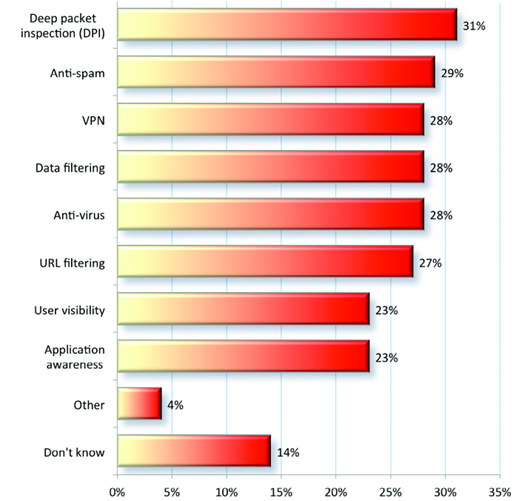
\includegraphics[width=0.6\textwidth]{Immagini/most_disable_feat_it_admin.png}
                \caption{Risposta a: “Quale funzionalità di sicurezza è disabilità per favorire le performance?” \cite{intel_sec_mcafee}.}
                \label{fig:disable_feat}
            \end{figure}

            Spesso i manager e i direttori operativi delle organizzazioni non sono al corrente dello stato di sicurezza delle loro reti, e lo scoprono quando è troppo tardi. Tra i vari reparti IT tutti vogliono supportare l'organizzazione dal punto di vista informatico, ma a volte alcune mansioni, come ad esempio la gestione delle regole del firewall, vengono assegnati a reparti che sottostimano i rischi di sicurezza, preferendo le performance.

            Un altro rischio che viene citato nel paper è quello dei BYOD, i quali possono essere punti di entrata per potenziali attaccanti. Per fare un esempio basta pensare agli attacchi di tipo AET, Advanced Evasion Techniques, attacchi sofisticati che usano diverse tecniche di evasione per rimanere inosservati nella rete per molto tempo; utilizzando tecniche come la frammentazione, bypassano gli IPS. Gli AET dividono il loro payload in piccoli pezzi che vengono consegnati contemporaneamente per poi venire riassemblati e completare l'attacco. Il 40\% degli addetti ai lavori ha sperimentato un attacco dove la tecnica AET ha giocato un ruolo chiave per la riuscita di quest'ultimo.

            Per risolvere questo problema bisognerebbe testare frequentemente la propria attrezzatura, assicurandosi di bilanciare correttamente la performance senza trascurare la sicurezza e collaborando tra i vari reparti IT per raggiungere questo compromesso. Inoltre i direttori operativi dovrebbero considerare di investire di più nella loro sicurezza, rendendo la loro rete scalabile per facilitare il compromesso tra sicurezza e prestazioni. Leggiamo nel paper menzionato come già aggiungere un NGFW a un cluster di 3 o più può incrementare le performance di almeno il 75\% e dovrebbero inserire delle routine organizzate per testare la loro rete più frequentemente.
